% !TeX root = RJwrapper.tex
\title{Finding Optimal Normalizing Transformations via
\pkg{bestNormalize}}
\author{by Ryan A. Peterson}

\maketitle

\abstract{%
The \pkg{bestNormalize} R package was designed to help users find a
transformation that can effectively normalize a vector regardless of its
actual distribution. Each of the many normalization techniques that have
been developed has its own strengths and weaknesses, and deciding which
to use until data are fully observed is difficult or impossible. This
package facilitates choosing between a range of possible transformations
and will automatically return the best one, i.e., the one that makes
data look the \emph{most} normal. To evaluate and compare the
normalization efficacy across a suite of possible transformations, we
developed a statistic based on a goodness of fit test divided by its
degrees of freedom. Transformations can be seamlessly trained and
applied to newly observed data and can be implemented in conjunction
with \pkg{caret} and \pkg{recipes} for data preprocessing in machine
learning workflows. Custom transformations and normalization statistics
are supported.
}

\hypertarget{introduction}{%
\section{Introduction}\label{introduction}}

The \CRANpkg{bestNormalize} package contains a suite of
transformation-estimating functions that can be used to normalize data.
The function of the same name attempts to find and execute the best of
all of these potential normalizing transformations. In this package, we
define ``normalize'' as in ``to render data Gaussian'', rather than
transform them to a specific scale.

There are many instances where researchers may want to normalize a
variable. First, there is the (often problematic) assumption of
normality of the outcome (conditional on the covariates) in the
classical linear regression problem. Over the years, many methods have
been used to relax this assumption: generalized linear models, quantile
regression, survival models, etc. One technique that is still somewhat
popular in this context is to ``beat the data'' to look normal via some
kind of normalizing transformation. This could be something as simple as
a log transformation or something as complex as a Yeo-Johnson
transformation \citep{yeojohnson}. In fact, many complex normalization
methods were designed expressly to find a transformation that could
render regression residuals Gaussian. While perhaps not the most elegant
solution to the problem, often, this technique works well as a quick
solution. Another increasingly popular application of normalization
occurs in applied regression settings with highly skewed distributions
of the covariates \citep{kuhn2013APM}. In these settings, there exists
the tendency to have high leverage points (and highly influential
points), even when one centers and scales the covariates. When examining
interactions, these influential points can become especially problematic
since the leverage of that point gets amplified for every interaction in
which it is involved. Normalization of such covariates can mitigate
their leverage and influence, thereby allowing for easier model
selection and more robust downstream predictor manipulations (such as
principal components analysis), which can otherwise be sensitive to skew
or outliers. As a result, popular model selection packages such as
\CRANpkg{caret} \citep{caret} and \CRANpkg{recipes} \citep{recipes} have
built-in mechanisms to normalize the predictor variables (they call this
``preprocessing''). This concept is unique in that it forgoes the
assumption of linearity between the outcome (Y) and the covariate,
opting instead for a linear relationship between Y and the transformed
value of the covariate (which in many cases may be more plausible).

This package is designed to make normalization effortless and
consistent. We have also introduced Ordered Quantile (ORQ) normalization
via the \code{orderNorm} function, which uses a rank mapping of the
observed data to the normal distribution~in order to guarantee normally
distributed transformed data (if ties are not present). We have shown
how ORQ normalization performs very consistently across different
distributions, successfully normalizing left- or right-skewed data,
multi-modal data, and even data generated from a Cauchy distribution
\citep{orq_paper}.

In this paper, we describe our R package \pkg{bestNormalize}, which is
available via the Comprehensive R Archive Network (CRAN). First, we
describe normalization methods that have been developed and that we
implement in the package. Second, we describe the novel
cross-validation-based estimation procedure, which we utilize to judge
the normalization efficacy of our suite of normalization
transformations. Third, we go through some basic examples of
\pkg{bestNormalize} functionality and a simple implementation of our
methods within the \pkg{recipes} package. We illustrate a more in-depth
use-case in a car pricing application, performing a transform-both-sides
regression as well as comparing the performance of several predictive
models fit via \pkg{caret}. Finally, we conclude by discussing the pros
and cons of normalization in general and future directions for the
package.

\hypertarget{normalization-methods}{%
\section{Normalization methods}\label{normalization-methods}}

Many normalization transformation functions exist, and though some can
be implemented well in existing R packages, \pkg{bestNormalize} puts
them all under the same umbrella syntax. This section describes each
transformation contained in the \pkg{bestNormalize} suite.

\hypertarget{the-box-cox-transformation}{%
\subsection{The Box-Cox
transformation}\label{the-box-cox-transformation}}

The Box-Cox transformation was famously proposed in \citet{BoxCox1964}
and can be implemented with differing syntax and methods in many
existing packages in R (e.g., \pkg{caret}, \CRANpkg{MASS} \citep{MASS},
and more). It is a straightforward transformation that typically only
involves one parameter, \(\lambda\):

\[
g(x; \lambda) = \boldsymbol 1 _{(\lambda \neq 0)} \frac{x^\lambda-1}{\lambda} 
+ \boldsymbol 1_{(\lambda = 0)} \log x\text{ ,}
\]

\noindent where \(x\) refers to the datum in its original unit
(pre-transformation). Given multiple observations, the \(\lambda\)
parameter can be estimated via maximum likelihood, and \(x\) must be
greater than zero.

\hypertarget{the-yeo-johnson-transformation}{%
\subsection{The Yeo-Johnson
transformation}\label{the-yeo-johnson-transformation}}

The Yeo-Johnson transformation \citep{yeojohnson} attempts to find the
value of \(\lambda\) in the following equation that minimizes the
Kullback-Leibler distance between the normal distribution and the
transformed distribution.

\[
\begin{aligned}
g(x;\lambda) &= 
\boldsymbol 1 _{(\lambda \neq 0, x \geq 0)} \frac{(x+1)^\lambda-1}{\lambda} \\
&+ \boldsymbol 1_{(\lambda = 0, x \geq 0)} \log (x+1) \\
&+ \boldsymbol 1_{(\lambda \neq 2, x < 0)} \frac{(1-x)^{2-\lambda}-1}{\lambda - 2} \\
&+ \boldsymbol 1_{(\lambda = 2, x < 0)} -\log (1-x) \\
\end{aligned}
\]

This method has the advantage of working without having to worry about
the domain of \(x\). As with the Box-Cox \(\lambda\), this \(\lambda\)
parameter can be estimated via maximum likelihood.

\hypertarget{the-lambert-w-x-f-transformation}{%
\subsection{The Lambert W x F
transformation}\label{the-lambert-w-x-f-transformation}}

The Lambert W x F transformation, proposed in \citet{goerg2011} and
implemented in the \CRANpkg{LambertW} package, is essentially a
mechanism that de-skews a random variable \(X\) using moments. The
method is motivated by a system theory and is alleged to be able to
transform any random variable into any other kind of random variable,
thus being applicable to a large number of contexts. One of the
package's main functions is \code{Gaussianize}, which is similar in
spirit to the purpose of this package. However, this method may not
perform as well on certain shapes of distributions as other candidate
transformations; see \citet{orq_paper} for some examples.

The \code{Gaussianize} transformation can handle three types of
transformations: skewed, heavy-tailed, and skewed heavy-tailed. For more
details on this transformation, consult the \pkg{LambertW}
documentation.\footnote{As of version 1.2.0 of \pkg{bestNormalize}, \code{lambert} methods are not performed by default in \code{bestNormalize}, but they are still available via the \code{allow\textunderscore lambert} arguments.}
While the transformations contained and implemented by
\code{bestNormalize} are reversible (i.e., 1-1), in rare circumstances,
we have observed that the \code{lambert} function can yield
non-reversible transformations.

\hypertarget{the-ordered-quantile-technique}{%
\subsection{The Ordered Quantile
technique}\label{the-ordered-quantile-technique}}

The ORQ normalization technique (\code{orderNorm}) is based on the
following transformation (originally discussed, as far as we can find,
in \citet{bartlett1947} and further developed in \citet{van1952}):

Let \(\underline x\) refer to the original data. Then the transformation
is:

\[
g(\underline x) = \Phi ^{-1} \left(\frac{\text{rank} (\underline x) - 1/2}{\text{length}(\underline x) }\right)
\]

This nonparametric transformation as defined works well on the observed
data, but it is not trivial to implement in modern settings where the
transformation needs to be applied on new data; we discussed this issue
and our solution to it in \citet{orq_paper}. Basically, on new data
\emph{within} the range of the original data, ORQ normalization will
linearly interpolate between two of the original data points. On new
data \emph{outside} the range of the original data, the transformation
extrapolates using a shifted logit approximation of the ranks to the
original data. This is visualized below via the \code{iris} data set on
the \code{Petal.Width} variable.

\begin{Schunk}
\begin{figure}

{\centering 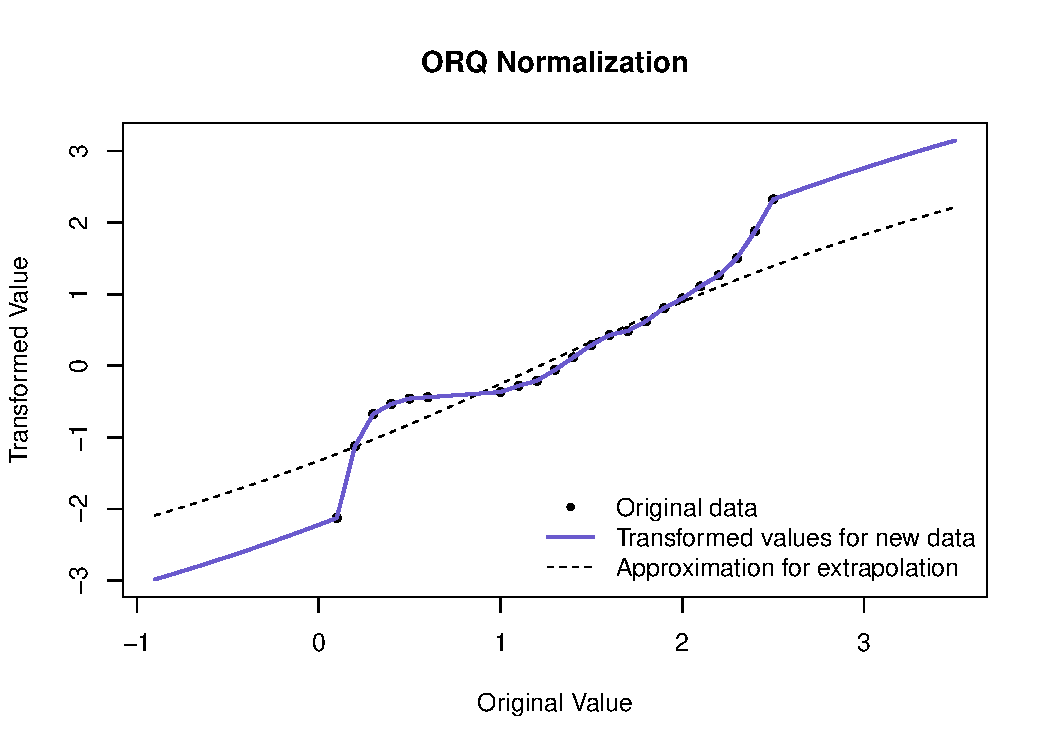
\includegraphics[width=1\linewidth]{figs/orq_vis-1} 

}

\caption[ORQ normalization visualization on Fisher's iris data]{ORQ normalization visualization on Fisher's iris data.}(\#fig:orq_vis)
\end{figure}
\end{Schunk}

The shifted logit extrapolation ensures that the function is 1-1 and can
handle data outside the original (observed) domain. The effects of the
approximation will usually be relatively minimal since we should not
expect to see many observations outside the observed range if the
training set sample size is large relative to the test set. The ORQ
technique will not guarantee a normal distribution in the presence of
ties, but it still could yield the best normalizing transformation when
compared to the other possible approaches. More information on ORQ
normalization can be found in \citet{orq_paper} or in the
\pkg{bestNormalize} documentation.

\hypertarget{other-included-transformations}{%
\subsection{Other included
transformations}\label{other-included-transformations}}

In addition to the techniques above, the \pkg{bestNormalize} package
performs and evaluates:

\begin{itemize}
\tightlist
\item
  \(\log_b(x + a)\) where \(a = \max(0, -\min(x) + \epsilon)\) and
  \(b = 10\) by default
\item
  \(\sqrt{x + a}\) where \(a = \max(0, -\min(x))\) by default
\item
  \(\exp(x)\)
\item
  \(\text {arcsinh}(x) = log(x + \sqrt{x^2 + 1})\)
\end{itemize}

\hypertarget{other-not-included-transformations}{%
\subsection{Other not-included
transformations}\label{other-not-included-transformations}}

A range of other normalization techniques has been proposed that are not
included in this package (at the time of writing). These include (but
are not limited to): Modified Box-Cox \citep{BoxCox1964}, Manly's
Exponential \citep{Manly}, John/Draper's Modulus \citep{JohnDraper}, and
Bickel/Doksum's Modified Box-Cox \citep{BickelDoksum}. However, it is
straightforward to add new transformations into the same framework as
other included transformations; each one is treated as its own S3 class,
so in order to add other transformations, all one must do is define a
new S3 class and provide the requisite S3 methods. To this end, we
encourage readers to submit a pull request to
\href{https://github.com/petersonR/bestNormalize}{the package's GitHub
page} with new transformation techniques that could be then added as a
default in \code{bestNormalize}. Otherwise, in a later section, we show
how users can implement custom transformations alongside the default
ones described above.

\hypertarget{which-transformation-best-normalizes-the-data}{%
\section{Which transformation ``best normalizes'' the
data?}\label{which-transformation-best-normalizes-the-data}}

The \code{bestNormalize} function selects the best transformation
according to an extra-sample estimate of the Pearson P statistic divided
by its degrees of freedom (\(DF\)). This P statistic is defined as

\[
P = \sum_{i=1}^{k} \frac{(O_i - E_i)^2}{E_i}\text{ ,}
\]

\noindent where \(O_i\) is the number observed, and \(E_i\) is the
number of expected (under the hypothesis of normality) to fall into
``bin'' \(i\). The bins (or ``classes'') are built such that
observations will fall into each one with equal probability under the
hypothesis of normality. A variety of alternative normality tests exist,
but this particular one is relatively interpretable as a goodness of fit
test, and the ratio \(P/DF\) can be compared between transformations as
an absolute measure of departure from normality. Specifically, if the
data in question follow a normal distribution, this ratio will be close
to 1 or lower. The transformation which produces data with the lowest
normality statistic is thus the most effective at normalizing the data,
and gets selected by \code{bestNormalize}. The \pkg{bestNormalize}
package utilizes \CRANpkg{nortest} \citep{nortest} to compute this
statistic; more information on its computation and degrees of freedom
can be found in \citet{d1986goodness} and \citet{thode2002testing}.

Normality statistics for all candidate transformations can be estimated
and compared with one simple call to \code{bestNormalize}, whose output
makes it easy to see which transformations are viable and which are not.
We have found that while complicated transformations are often
\emph{most} effective and therefore selected automatically, sometimes a
simple transformation (e.g., the log or identity transforms) may be
almost as effective, and ultimately the latter type will yield more
interpretable results.

It is worth noting that when the normality statistic is estimated on
in-sample data, the ORQ technique is predestined to be most effective
since it is forcing its transformed data to follow a normal distribution
exactly \citep{orq_paper}. For this reason, by default, the
\code{bestNormalize} function calculates an \emph{out-of-sample}
estimate for the \(P/DF\) statistic. Since this method necessitates
cross-validation, it can be computationally frustrating for three
reasons: (1) the results and the chosen transformation can depend on the
seed, (2) it takes considerably longer to estimate than the in-sample
statistic, and (3) it is unclear how to choose the number of folds and
repeats.

In order to mediate these issues, we have built several features into
\pkg{bestNormalize}. Issue (1) is only important for small sample sizes,
and when it is a concern, the best transformations should look similar
to one another. We address two solutions to (2) in the next section. In
short, we have methods to parallelize or simplify the estimation of the
statistic. For (3), we recommend 10-fold cross-validation with 5 repeats
as the default, but if the sample is small, we suggest using 5 (or
fewer) folds instead with more repeats; accurate estimation of \(P/DF\)
requires a relatively large fold size (as a rule of thumb, 20
observations per fold seems to be enough for most cases, but this
unfortunately depends on the distribution of the observed data).

\hypertarget{simple-examples}{%
\section{Simple examples}\label{simple-examples}}

In this section, we illustrate a simple use-case of the functions
provided in \pkg{bestNormalize}.

\hypertarget{basic-implementation}{%
\subsection{Basic implementation}\label{basic-implementation}}

First, we will generate and plot some skewed data:

\begin{Schunk}
\begin{Sinput}
x <- rgamma(250, 1, 1)
\end{Sinput}
\end{Schunk}

\begin{Schunk}
\begin{figure}

{\centering 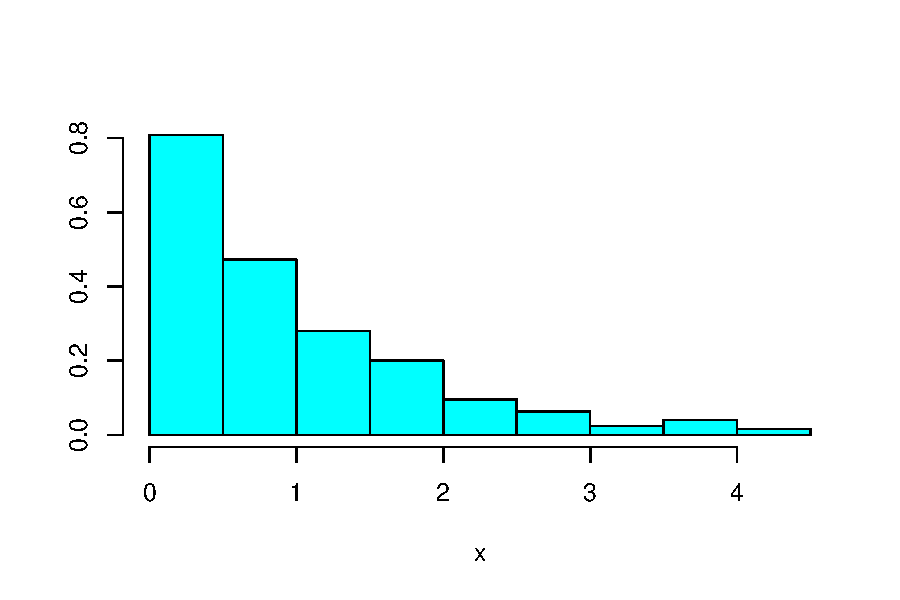
\includegraphics[width=2.5in,height=1.3in]{figs/simple_hist-1} 

}

\caption[Simulated skewed data for simple example]{Simulated skewed data for simple example.}(\#fig:simple_hist)
\end{figure}
\end{Schunk}

To perform a suite of potential transformations and see how effectively
they normalized this vector, simply call \code{bestNormalize}:

\begin{Schunk}
\begin{Sinput}
(BNobject <- bestNormalize(x))
\end{Sinput}
\begin{Soutput}
#> Best Normalizing transformation with 250 Observations
#>  Estimated Normality Statistics (Pearson P / df, lower => more normal):
#>  - arcsinh(x): 1.7917
#>  - Box-Cox: 1.0442
#>  - Center+scale: 3.0102
#>  - Exp(x): 9.5306
#>  - Log_b(x+a): 1.7072
#>  - orderNorm (ORQ): 1.1773
#>  - sqrt(x + a): 1.144
#>  - Yeo-Johnson: 1.1875
#> Estimation method: Out-of-sample via CV with 10 folds and 5 repeats
#>  
#> Based off these, bestNormalize chose:
#> Standardized Box Cox Transformation with 250 nonmissing obs.:
#>  Estimated statistics:
#>  - lambda = 0.3254863 
#>  - mean (before standardization) = -0.3659267 
#>  - sd (before standardization) = 0.9807881
\end{Soutput}
\end{Schunk}

Evidently, the Box-Cox transformation performed the best, though many
other transformations performed similarly. We can visualize the suite of
transformations using the built-in \code{plot} method:

\begin{Schunk}
\begin{Sinput}
plot(BNobject, leg_loc = "topleft")
\end{Sinput}
\begin{figure}

{\centering 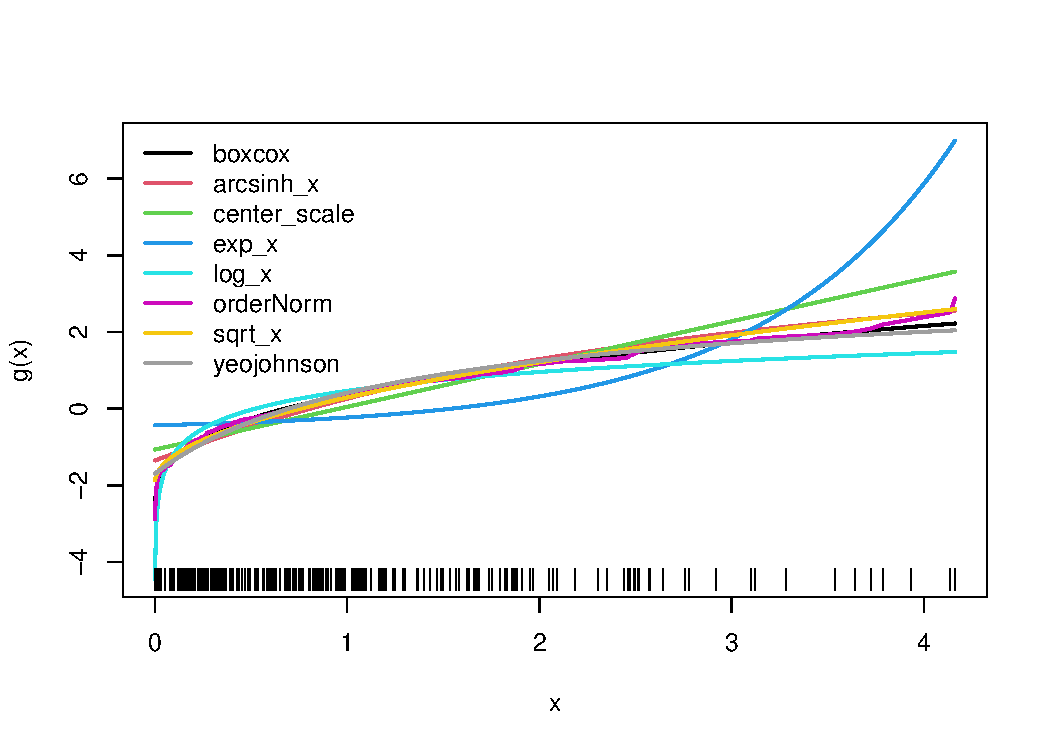
\includegraphics[width=1\linewidth]{figs/bn_plot-1} 

}

\caption[The suite of transformations estimated by default in \pkg{bestNormalize} (trained on simulated right-skewed data)]{The suite of transformations estimated by default in \pkg{bestNormalize} (trained on simulated right-skewed data).}(\#fig:bn_plot)
\end{figure}
\end{Schunk}

Finally, we can execute the best performing normalization on new data
with \code{predict(BNobject,\ new\textunderscore x)} or reverse the
transformation with
\code{predict(BNobject,\ new\textunderscore x\textunderscore t, inverse = TRUE)}.
Note that normalized values can either be obtained using \code{predict}
or by extracting \code{x.t} from the object. The best transformation, in
this case, is plotted in Figure 4.

\begin{Schunk}
\begin{figure}

{\centering 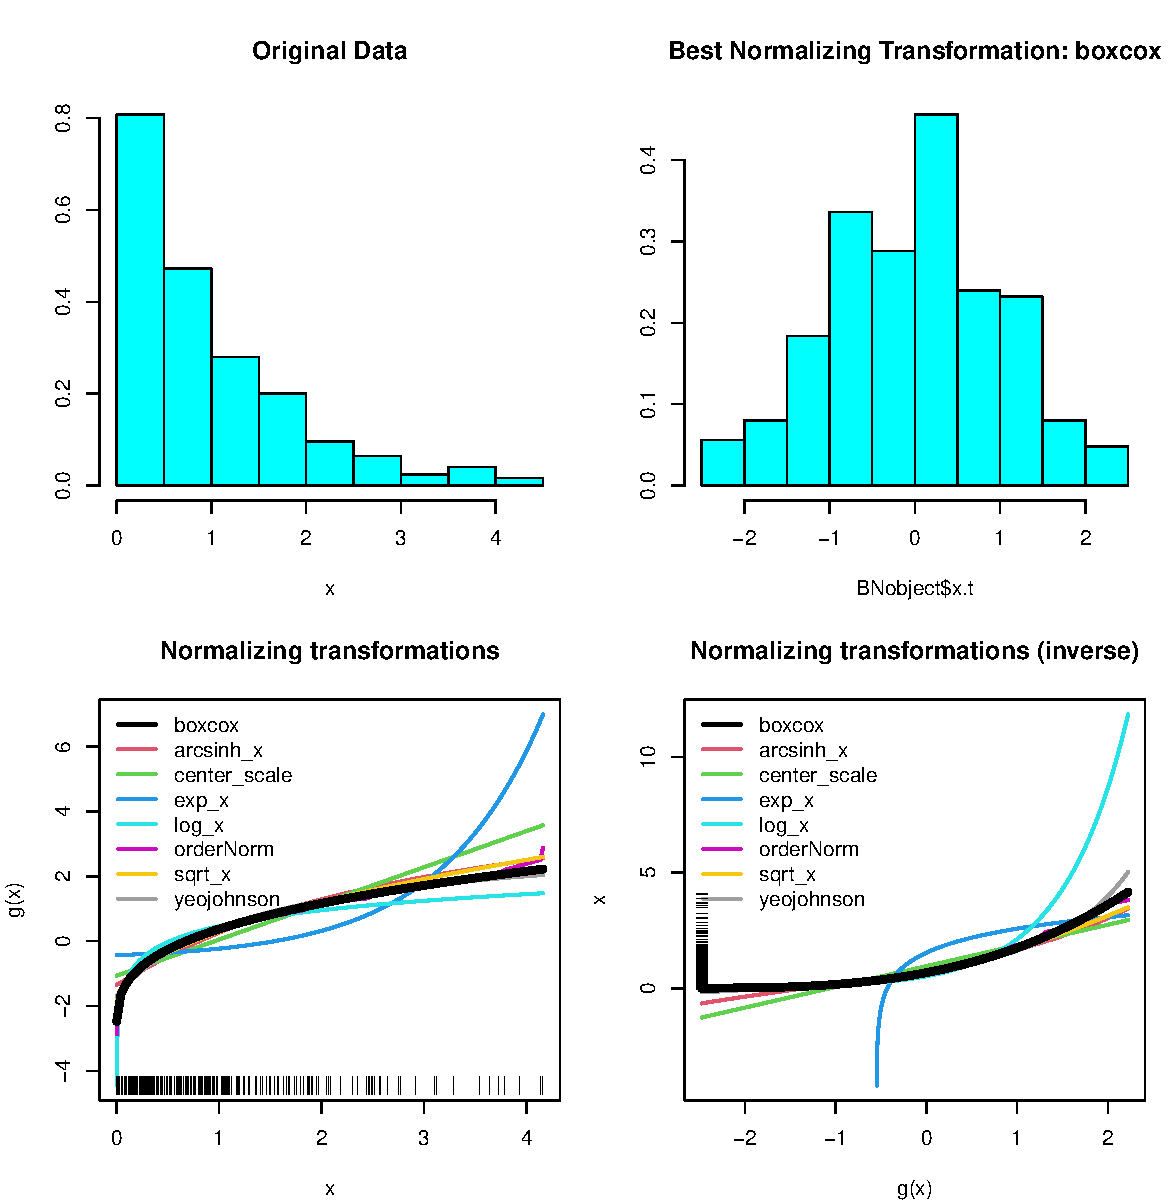
\includegraphics[width=1\linewidth]{figs/hist_best-1} 

}

\caption[Summary of transformations performed on simulated right-skewed data]{Summary of transformations performed on simulated right-skewed data.}(\#fig:hist_best)
\end{figure}
\end{Schunk}

\hypertarget{performing-transformations-individually}{%
\subsection{Performing transformations
individually}\label{performing-transformations-individually}}

Each method can be performed (and stored) individually:

\begin{Schunk}
\begin{Sinput}
(arcsinh_obj <- arcsinh_x(x))
\end{Sinput}
\begin{Soutput}
#> Standardized asinh(x) Transformation with 250 nonmissing obs.:
#>  Relevant statistics:
#>  - mean (before standardization) = 0.7383146 
#>  - sd (before standardization) = 0.5458515
\end{Soutput}
\begin{Sinput}
(boxcox_obj <- boxcox(x))
\end{Sinput}
\begin{Soutput}
#> Standardized Box Cox Transformation with 250 nonmissing obs.:
#>  Estimated statistics:
#>  - lambda = 0.3254863 
#>  - mean (before standardization) = -0.3659267 
#>  - sd (before standardization) = 0.9807881
\end{Soutput}
\begin{Sinput}
(yeojohnson_obj <- yeojohnson(x))
\end{Sinput}
\begin{Soutput}
#> Standardized Yeo-Johnson Transformation with 250 nonmissing obs.:
#>  Estimated statistics:
#>  - lambda = -0.7080476 
#>  - mean (before standardization) = 0.4405464 
#>  - sd (before standardization) = 0.2592004
\end{Soutput}
\begin{Sinput}
(lambert_obj <- lambert(x, type = "s"))
\end{Sinput}
\begin{Soutput}
#> Standardized Lambert WxF Transformation of type s with 250 nonmissing obs.:
#>  Estimated statistics:
#>  - gamma = 0.3729
#>  - mean (before standardization) = 0.6781864 
#>  - sd (before standardization) = 0.7123011
\end{Soutput}
\begin{Sinput}
(orderNorm_obj <- orderNorm(x))
\end{Sinput}
\begin{Soutput}
#> orderNorm Transformation with 250 nonmissing obs and no ties 
#>  - Original quantiles:
#>    0%   25%   50%   75%  100% 
#> 0.001 0.268 0.721 1.299 4.161
\end{Soutput}
\end{Schunk}

All normalization techniques in \code{bestNormalize} have their own
class with convenient S3 methods and documentation. For instance, we can
use the \code{predict} method to perform the transformation on new
values using the objects we have just created, visualizing them in a
plot:

\begin{Schunk}
\begin{Sinput}
xx <- seq(min(x), max(x), length = 100)
plot(xx, predict(arcsinh_obj, newdata = xx), type = "l", col = 1)
lines(xx, predict(boxcox_obj, newdata = xx), col = 2)
lines(xx, predict(yeojohnson_obj, newdata = xx), col = 3)
lines(xx, predict(orderNorm_obj, newdata = xx), col = 4)
\end{Sinput}
\end{Schunk}

\begin{Schunk}
\begin{figure}

{\centering 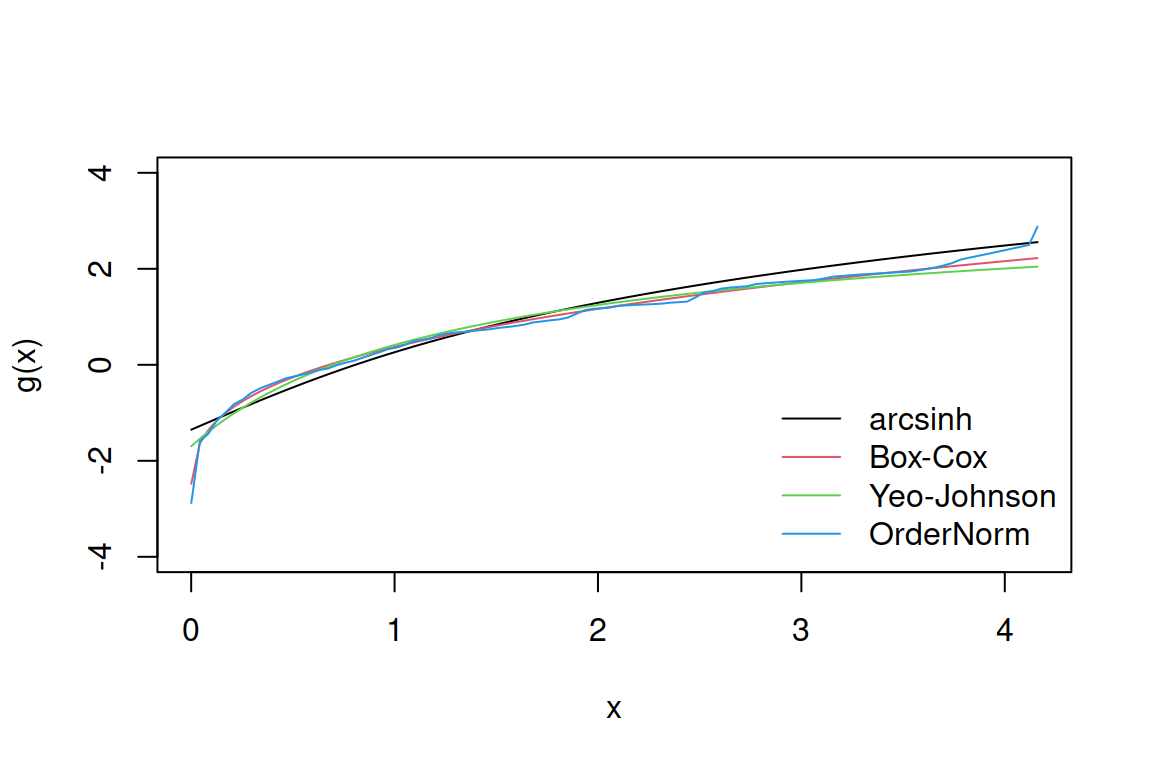
\includegraphics[width=4.375in,height=2.5in]{figs/vis_data2-1} 

}

\caption[Manually plotting transformations trained on simulated right-skewed data]{Manually plotting transformations trained on simulated right-skewed data.}(\#fig:vis_data2)
\end{figure}
\end{Schunk}

\hypertarget{in-sample-normalization-efficacy}{%
\subsection{In-sample normalization
efficacy}\label{in-sample-normalization-efficacy}}

To examine how each of the normalization methods performed (in-sample),
we can visualize the transformed values in histograms (Figure 6), which
plot the transformed data, \code{x.t}, stored in the transformation
objects we created previously.

\begin{Schunk}
\begin{figure}

{\centering 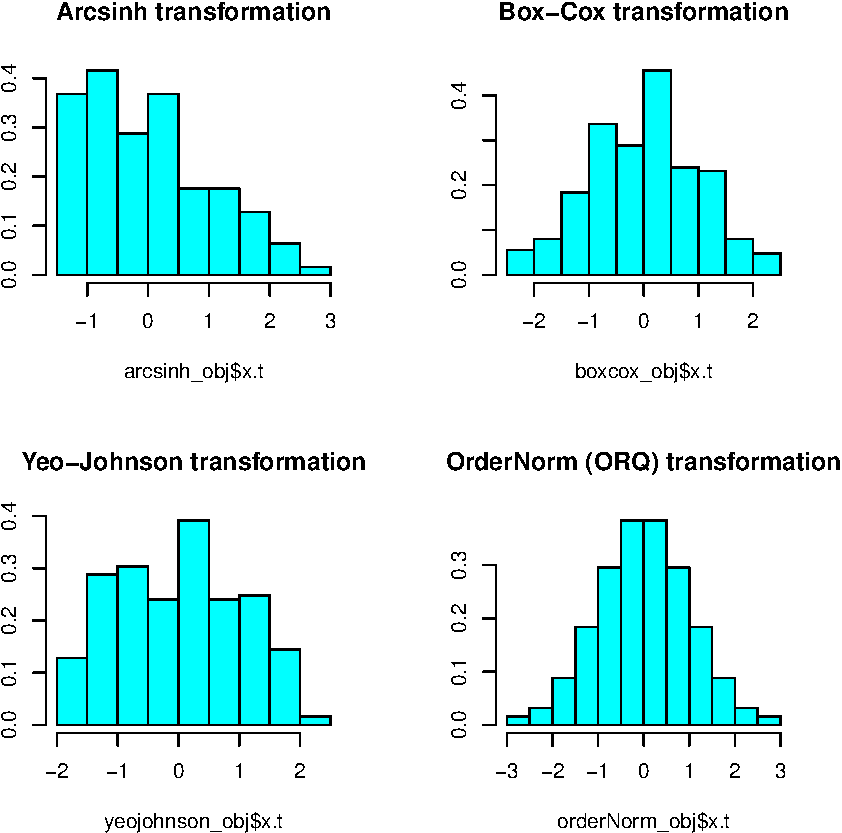
\includegraphics[width=4in,height=4in]{figs/hist_trans-1} 

}

\caption[Normalized values for trained transformations on simulated right-skewed data]{Normalized values for trained transformations on simulated right-skewed data.}(\#fig:hist_trans)
\end{figure}
\end{Schunk}

Evidently, ORQ normalization appears to have worked perfectly to
normalize the data (as expected), and the Box-Cox method seemed to do
quite well too.

\hypertarget{out-of-sample-normalization-efficacy}{%
\subsection{Out-of-sample normalization
efficacy}\label{out-of-sample-normalization-efficacy}}

The \code{bestNormalize} function performs repeated (r=5) 10-fold
cross-validation (CV) by default and stores the estimated normality
statistic for each left-out fold/repeat into
\code{oos\textunderscore preds}. Users can access and visualize these
results via a boxplot (see below), which may give some insight into
whether the transformation is truly preferred by the normality statistic
or if another (possibly simpler) transformation can be applied that
would achieve the approximately the same results. In this example,
Box-Cox, square-root, Yeo-Johnson, and ORQ seem to do similarly well,
whereas the identity
transform\footnote{Since \code{standardize=TRUE}, the identity transformation is represented in Figure 7 by \code{center\textunderscore scale}, which yields the exact same normality statistic.},
hyperbolic arc-sine, logging, and exponentiation are performing worse.

\begin{Schunk}
\begin{Sinput}
boxplot(BNobject$oos_preds, log = 'y')
abline(h = 1, col = "green3")
\end{Sinput}
\begin{figure}

{\centering 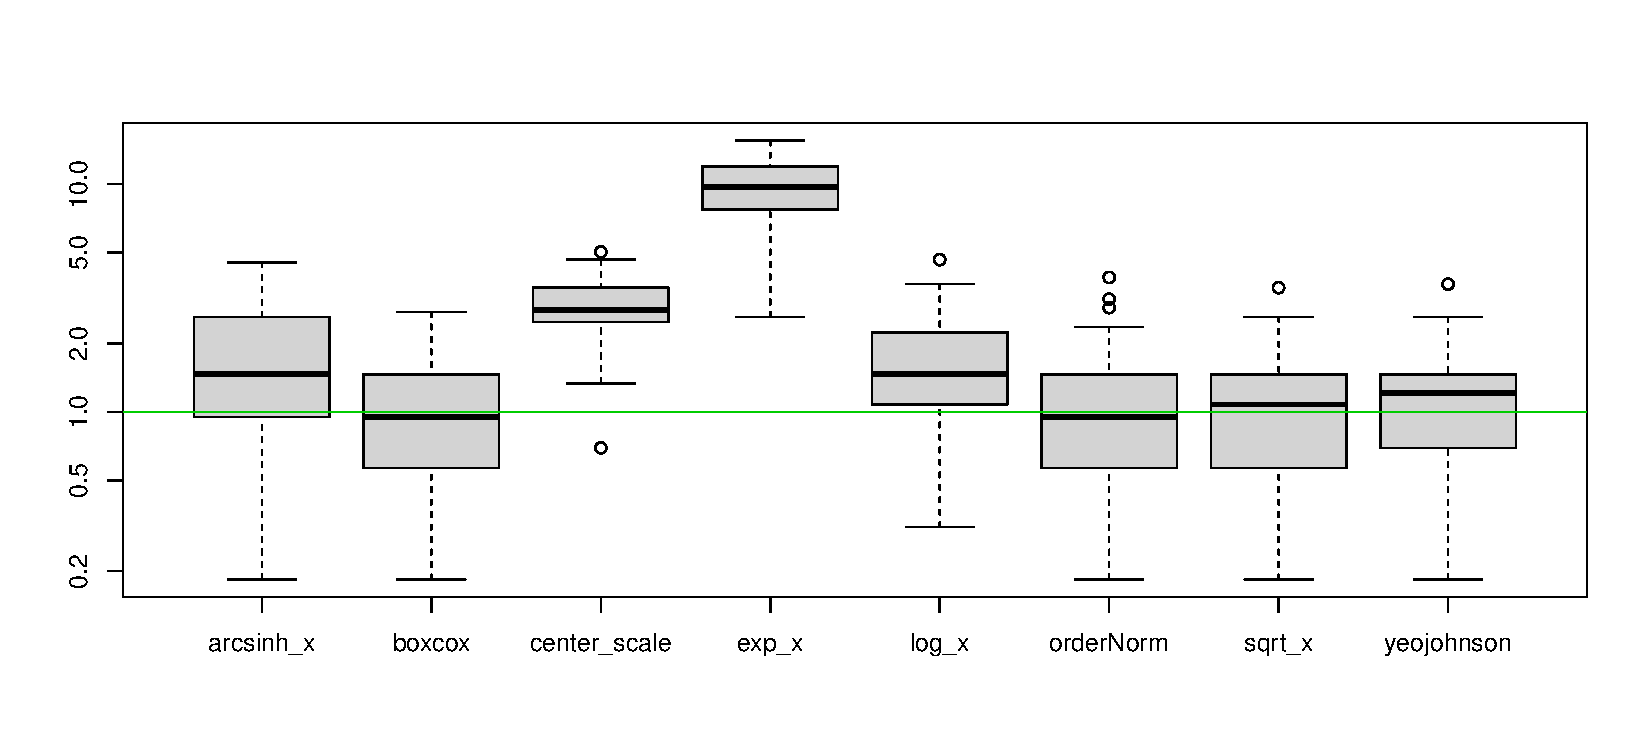
\includegraphics[width=1\linewidth]{figs/boxplot-1} 

}

\caption[Cross-validation results for each normalization method, where our estimated normality statistic is plotted on the y-axis]{Cross-validation results for each normalization method, where our estimated normality statistic is plotted on the y-axis.}(\#fig:boxplot)
\end{figure}
\end{Schunk}

Leave-one-out CV can be optionally performed in \code{bestNormalize} via
the \code{loo} argument, which, if set to \code{TRUE}, will compute the
leave-one-out CV transformations for each observation and method.
Specifically, \code{bestNormalize} will be run \(n\) separate times
where each observation is individually left out of the fitting process
and subsequently plugged back in to get a ``leave-one-out transformed
value''. Instead of taking the mean across repeats and folds, in this
case, we estimate normalization efficacy using the full distribution of
leave-one-out transformed values. This option is computationally
intensive. Note that as with the ``in-sample'' normality statistics, the
leave-one-out CV approach tends to select the ORQ transformation since
ORQ's performance improves as the number of points in the training set
relative to the testing set increases.

\begin{Schunk}
\begin{Sinput}
bestNormalize(x, loo = TRUE)
\end{Sinput}
\begin{Soutput}
#> Best Normalizing transformation with 250 Observations
#>  Estimated Normality Statistics (Pearson P / df, lower => more normal):
#>  - arcsinh(x): 4.42
#>  - Box-Cox: 0.7055
#>  - Center+scale: 8.258
#>  - Exp(x): 62.085
#>  - Log_b(x+a): 3.546
#>  - orderNorm (ORQ): 0.012
#>  - sqrt(x + a): 0.9145
#>  - Yeo-Johnson: 1.608
#> Estimation method: Out-of-sample via leave-one-out CV
#>  
#> Based off these, bestNormalize chose:
#> orderNorm Transformation with 250 nonmissing obs and no ties 
#>  - Original quantiles:
#>    0%   25%   50%   75%  100% 
#> 0.001 0.268 0.721 1.299 4.161
\end{Soutput}
\end{Schunk}

\hypertarget{important-features}{%
\section{Important features}\label{important-features}}

\hypertarget{improving-speed-of-estimation}{%
\subsection{Improving speed of
estimation}\label{improving-speed-of-estimation}}

Because \code{bestNormalize} uses repeated CV by default to estimate the
out-of-sample normalization efficacy, it can be quite slow for larger
objects. There are several means of speeding up the process. Each comes
with some pros and cons. The first option is to specify
\code{out\textunderscore of\textunderscore sample = FALSE}. This will
highly speed up the process. However, for reasons previously discussed,
ORQ normalization will always be chosen unless
\code{allow\textunderscore orderNorm = FALSE}. Therefore, a user might
as well use the \code{orderNorm} function directly as opposed to only
setting \code{out\textunderscore of\textunderscore sample = FALSE} since
the end result will be the same (and \code{orderNorm} will run much
faster). Note below that the in-sample normality results may differ
slightly from the leave-one-out even when this may be unexpected (i.e.,
for the log transformation); this is due to slight differences in the
standardization statistics.

\begin{Schunk}
\begin{Sinput}
bestNormalize(x, allow_orderNorm = FALSE, out_of_sample = FALSE)
\end{Sinput}
\begin{Soutput}
#> Best Normalizing transformation with 250 Observations
#>  Estimated Normality Statistics (Pearson P / df, lower => more normal):
#>  - arcsinh(x): 4.401
#>  - Box-Cox: 0.7435
#>  - Center+scale: 8.087
#>  - Exp(x): 64.6975
#>  - Log_b(x+a): 3.47
#>  - sqrt(x + a): 0.9145
#>  - Yeo-Johnson: 1.7125
#> Estimation method: In-sample
#>  
#> Based off these, bestNormalize chose:
#> Standardized Box Cox Transformation with 250 nonmissing obs.:
#>  Estimated statistics:
#>  - lambda = 0.3254863 
#>  - mean (before standardization) = -0.3659267 
#>  - sd (before standardization) = 0.9807881
\end{Soutput}
\end{Schunk}

Another option to improve estimation efficiency is to use the built-in
parallelization functionality. The repeated CV process can be
parallelized via the \code{cluster} argument and the \CRANpkg{parallel}
and \CRANpkg{doRNG} \citep{doRNG} packages. A cluster can be set up with
\code{makeCluster} and passed to \code{bestNormalize} via the
\code{cluster = } argument.

\begin{Schunk}
\begin{Sinput}
cl <- parallel::makeCluster(5)
b <- bestNormalize(x, cluster = cl, r = 10, quiet = TRUE)
parallel::stopCluster(cl)
\end{Sinput}
\end{Schunk}

The amount by which this parallelization will speed up the estimation of
out-of-sample estimates depends (for the most part) on the number of
repeats, the number of cores, and the sample size of the vector to be
normalized. The plot below shows the estimation time for a run of
\code{bestNormalize} with 15 repeats of 10-fold CV on a
gamma-distributed random variable with various sample sizes and numbers
of cores.

\begin{Schunk}
\begin{figure}

{\centering 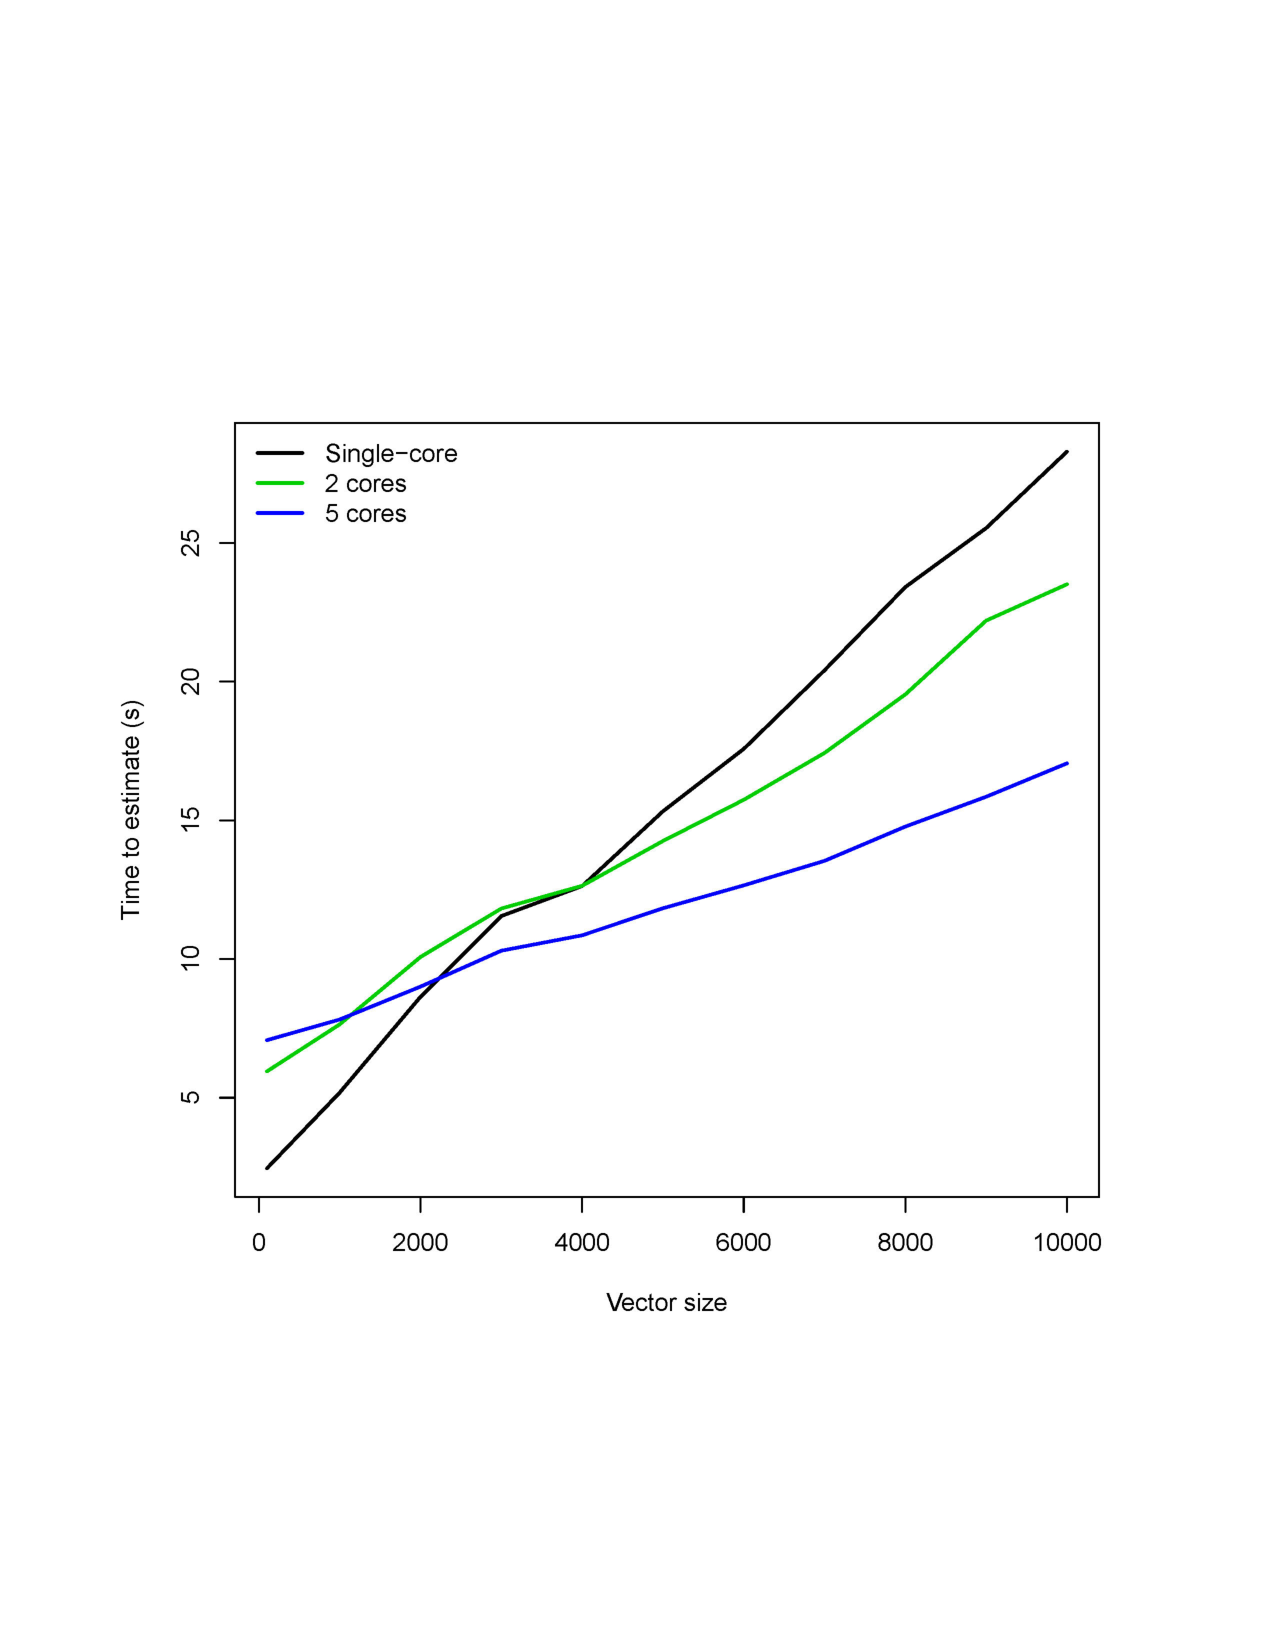
\includegraphics[width=1\linewidth]{figs/parallel_timings} 

}

\caption[Potential speedup using parallelization functionality]{Potential speedup using parallelization functionality.}(\#fig:parallel_timings)
\end{figure}
\end{Schunk}

\hypertarget{implementation-with-caret-recipes}{%
\subsection{Implementation with caret,
recipes}\label{implementation-with-caret-recipes}}

The \code{step\textunderscore best\textunderscore normalize} and the
\code{step\textunderscore orderNorm} functions can be utilized in
conjunction with the \pkg{recipes} package to preprocess data in machine
learning workflows with \CRANpkg{tidymodels} \citep{tidymodels} or in
combination with \pkg{caret}. The basic usage within \pkg{recipes} is
shown below; for implementation with \pkg{caret}, refer to this paper's
application.

\begin{Schunk}
\begin{Sinput}
rec <- recipe( ~ ., data = iris)  %>%                       # Initialize recipe
  step_best_normalize(all_predictors(), -all_nominal()) %>% # Transform predictors
  prep(iris) %>%                                            # Prep (train) recipe
  bake(iris)                                                # Bake (apply) recipe
\end{Sinput}
\end{Schunk}

Options can be supplied to
\code{step\textunderscore best\textunderscore normalize} to speed up or
alter performance via the \code{transform\textunderscore options}
argument, which passes a list of options to \code{bestNormalize}.

\hypertarget{additional-customization}{%
\subsection{Additional customization}\label{additional-customization}}

Two important means of customization are available: 1) users may add
custom transformation functions to be assessed alongside the default
suite of normalization methods, and 2) users may change the statistic
used ``under the hood'' by \code{bestNormalize} to estimate the
departure from normality of the transformed data. This section contains
examples and guidance for both extensions.

\hypertarget{adding-user-defined-functions}{%
\subsubsection{1) Adding user-defined
functions}\label{adding-user-defined-functions}}

Via the \code{new\textunderscore transforms} argument, users can use
\code{bestNormalize}'s machinery to compare custom, user-defined
transformation functions to those included in the package. Below, I
consider an example where a user may wish to compare the cube-root
function with those provided in the package. \code{bestNormalize}
requires two functions to implement this: the transformation function
and an associated \code{predict} method. The custom cube-root
transformation shown below is simple, but its skeleton can readily be
made arbitrarily more complex.

\begin{Schunk}
\begin{Sinput}
## Define custom function
cuberoot_x <- function(x, ...) {
  x.t <- (x)^(1/3)
  
  # Get in-sample normality statistic results
  ptest <- nortest::pearson.test(x.t)
  
  val <- list(
    x.t = x.t,
    x = x,
    n = length(x.t) - sum(is.na(x)), 
    norm_stat = unname(ptest$statistic / ptest$df)
  )
  
  # Assign class, return
  class(val) <- c('cuberoot_x')
  val
}

# S3 method that is used to apply the transformation to newly observed data
predict.cuberoot_x <- function(object, newdata = NULL, inverse = FALSE, ...) {
  
  # If no data supplied and not inverse
  if (is.null(newdata) & !inverse)
    newdata <- object$x
  
  # If no data supplied and inverse transformation is requested
  if (is.null(newdata) & inverse)
    newdata <- object$x.t
  
  # Perform inverse transformation
  if (inverse) {
    # Reverse-cube-root (cube)
    val <-  newdata^3
    
    # Otherwise, perform transformation as estimated
  } else if (!inverse) {
    val <- (newdata)^(1/3)
  }
  
  # Return transformed data
  unname(val)
}

## Optional: print S3 method
print.cuberoot_x <- function(x, ...) {
  cat('cuberoot(x) Transformation with', x$n, 'nonmissing obs.\n')
}
\end{Sinput}
\end{Schunk}

\noindent These functions can then be passed as a named list to
\code{bestNormalize}:

\begin{Schunk}
\begin{Sinput}
custom_transform <- list(
  cuberoot_x = cuberoot_x,
  predict.cuberoot_x = predict.cuberoot_x,
  print.cuberoot_x = print.cuberoot_x
)

set.seed(123129)
x <- rgamma(100, 1, 1)
(b <- bestNormalize(x = x, new_transforms = custom_transform))
\end{Sinput}
\begin{Soutput}
#> Best Normalizing transformation with 100 Observations
#>  Estimated Normality Statistics (Pearson P / df, lower => more normal):
#>  - arcsinh(x): 1.2347
#>  - Box-Cox: 1.0267
#>  - Center+scale: 2.0027
#>  - cuberoot_x: 0.9787
#>  - Exp(x): 4.7947
#>  - Log_b(x+a): 1.3547
#>  - orderNorm (ORQ): 1.1627
#>  - sqrt(x + a): 1.0907
#>  - Yeo-Johnson: 1.0987
#> Estimation method: Out-of-sample via CV with 10 folds and 5 repeats
#>  
#> Based off these, bestNormalize chose:
#> cuberoot(x) Transformation with 100 nonmissing obs.
\end{Soutput}
\end{Schunk}

Evidently, the cube-root was the best normalizing transformation for
this gamma-distributed random variable, performing comparably to the
Box-Cox transformation.

\hypertarget{re-defining-normality}{%
\subsubsection{2) Re-defining normality}\label{re-defining-normality}}

The question ``what is normal?'' outside of a statistical discussion is
quite loaded and subjective. Even in statistical discussions, many
authors have contributed to the question of how to best detect
departures from normality; these solutions are diverse, and several have
been implemented well in \pkg{nortest} already. In order to accommodate
those with varying opinions on the best definition of normality, we have
included a feature that allows users to specify a custom definition of a
normality statistic. This customization can be accomplished via the
\code{norm\textunderscore stat\textunderscore fn} argument, which takes
a function that will then be applied in lieu of the Pearson test
statistic divided by its degree of freedom to assess normality.

The user-defined function must take an argument \code{x}, which
indicates the data on which a user wants to evaluate the statistic.

Here is an example using the Lilliefors (Kolmogorov-Smirnov) normality
test statistic:

\begin{Schunk}
\begin{Sinput}
bestNormalize(x, norm_stat_fn = function(x) nortest::lillie.test(x)$stat)
\end{Sinput}
\begin{Soutput}
#> Best Normalizing transformation with 100 Observations
#>  Estimated Normality Statistics (using custom normalization statistic)
#>  - arcsinh(x): 0.1958
#>  - Box-Cox: 0.1785
#>  - Center+scale: 0.2219
#>  - Exp(x): 0.3299
#>  - Log_b(x+a): 0.1959
#>  - orderNorm (ORQ): 0.186
#>  - sqrt(x + a): 0.1829
#>  - Yeo-Johnson: 0.1872
#> Estimation method: Out-of-sample via CV with 10 folds and 5 repeats
#>  
#> Based off these, bestNormalize chose:
#> Standardized Box Cox Transformation with 100 nonmissing obs.:
#>  Estimated statistics:
#>  - lambda = 0.3281193 
#>  - mean (before standardization) = -0.1263882 
#>  - sd (before standardization) = 0.9913552
\end{Soutput}
\end{Schunk}

Here is an example using the Lillifors (Kolmogorov-Smirnov) normality
test's \textit{p}-value:

\begin{Schunk}
\begin{Sinput}
(dont_do_this <- bestNormalize(x, norm_stat_fn = function(x) nortest::lillie.test(x)$p))
\end{Sinput}
\begin{Soutput}
#> Best Normalizing transformation with 100 Observations
#>  Estimated Normality Statistics (using custom normalization statistic)
#>  - arcsinh(x): 0.4327
#>  - Box-Cox: 0.4831
#>  - Center+scale: 0.2958
#>  - Exp(x): 0.0675
#>  - Log_b(x+a): 0.3589
#>  - orderNorm (ORQ): 0.4492
#>  - sqrt(x + a): 0.4899
#>  - Yeo-Johnson: 0.4531
#> Estimation method: Out-of-sample via CV with 10 folds and 5 repeats
#>  
#> Based off these, bestNormalize chose:
#> Standardized exp(x) Transformation with 100 nonmissing obs.:
#>  Relevant statistics:
#>  - mean (before standardization) = 6.885396 
#>  - sd (before standardization) = 13.66084
\end{Soutput}
\end{Schunk}

Note: \code{bestNormalize} will attempt to minimize this statistic by
default, which is definitely not what you want to do when calculating
the \textit{p}-value. This is seen in the example above, where the
\textbf{worst} normalization transformation, exponentiation, is chosen.
In this case, a user is advised to either manually select the best one
or reverse their defined normalization statistic (in this case by
subtracting it from 1):

\begin{Schunk}
\begin{Sinput}
best_transform <- names(which.max(dont_do_this$norm_stats))
do_this <- dont_do_this$other_transforms[[best_transform]]
or_this <- bestNormalize(x, norm_stat_fn = function(x) 1-nortest::lillie.test(x)$p)
\end{Sinput}
\end{Schunk}

A \textit{p}-value for normality should not be routinely used as the
sole selector of a normalizing transformation. A normality test's
\textit{p}-value, as a measure of the departure from normality, is
confounded by the sample size (a high sample size may yield strong
evidence of a practically insignificant departure from normality).
Therefore, we suggest the statistic used should estimate the departure
from normality rather the strength of evidence against normality
\citep[e.g.,][]{normality}.

\hypertarget{application-to-autotrader-data}{%
\section{Application to Autotrader
data}\label{application-to-autotrader-data}}

\hypertarget{background}{%
\subsection{Background}\label{background}}

The \code{autotrader} data set was scraped from the
\href{https://www.autotrader.com/}{autotrader website} as part of this
package (and because at the time of data collection in 2017, the package
author needed to purchase a car). We apply the \pkg{bestNormalize}
functionality to de-skew mileage, age, and price in a pricing model. See
\code{?autotrader} for more information on this data set.

\begin{Schunk}
\begin{Sinput}
data("autotrader")
autotrader$yearsold <- 2017 - autotrader$Year
\end{Sinput}
\end{Schunk}

\begin{Schunk}
<table class="table table-striped table-condensed" style="width: auto !important; margin-left: auto; margin-right: auto;">
<caption>(\#tab:unnamed-chunk-10)Sample characteristics of `autotrader` data.</caption>
 <thead>
  <tr>
   <th style="text-align:left;">  </th>
   <th style="text-align:left;"> Overall (N=6,283) </th>
  </tr>
 </thead>
<tbody>
  <tr>
   <td style="text-align:left;"> Make </td>
   <td style="text-align:left;">  </td>
  </tr>
  <tr>
   <td style="text-align:left;"> -  Acura </td>
   <td style="text-align:left;"> 185 (2.9%) </td>
  </tr>
  <tr>
   <td style="text-align:left;"> -  Buick </td>
   <td style="text-align:left;"> 252 (4.0%) </td>
  </tr>
  <tr>
   <td style="text-align:left;"> -  Chevrolet </td>
   <td style="text-align:left;"> 1,257 (20.0%) </td>
  </tr>
  <tr>
   <td style="text-align:left;"> -  GMC </td>
   <td style="text-align:left;"> 492 (7.8%) </td>
  </tr>
  <tr>
   <td style="text-align:left;"> -  Honda </td>
   <td style="text-align:left;"> 1,029 (16.4%) </td>
  </tr>
  <tr>
   <td style="text-align:left;"> -  Hyundai </td>
   <td style="text-align:left;"> 381 (6.1%) </td>
  </tr>
  <tr>
   <td style="text-align:left;"> -  Mazda </td>
   <td style="text-align:left;"> 272 (4.3%) </td>
  </tr>
  <tr>
   <td style="text-align:left;"> -  Nissan </td>
   <td style="text-align:left;"> 735 (11.7%) </td>
  </tr>
  <tr>
   <td style="text-align:left;"> -  Pontiac </td>
   <td style="text-align:left;"> 63 (1.0%) </td>
  </tr>
  <tr>
   <td style="text-align:left;"> -  Toyota </td>
   <td style="text-align:left;"> 1,202 (19.1%) </td>
  </tr>
  <tr>
   <td style="text-align:left;"> -  Volkswagen </td>
   <td style="text-align:left;"> 415 (6.6%) </td>
  </tr>
  <tr>
   <td style="text-align:left;"> Price ($) </td>
   <td style="text-align:left;">  </td>
  </tr>
  <tr>
   <td style="text-align:left;"> -  Mean (SD) </td>
   <td style="text-align:left;"> 17,145 (8,346) </td>
  </tr>
  <tr>
   <td style="text-align:left;"> -  Range </td>
   <td style="text-align:left;"> 722 - 64,998 </td>
  </tr>
  <tr>
   <td style="text-align:left;"> Mileage </td>
   <td style="text-align:left;">  </td>
  </tr>
  <tr>
   <td style="text-align:left;"> -  Mean (SD) </td>
   <td style="text-align:left;"> 63,638 (49,125) </td>
  </tr>
  <tr>
   <td style="text-align:left;"> -  Range </td>
   <td style="text-align:left;"> 2 - 325,556 </td>
  </tr>
  <tr>
   <td style="text-align:left;"> Year </td>
   <td style="text-align:left;">  </td>
  </tr>
  <tr>
   <td style="text-align:left;"> -  Mean (SD) </td>
   <td style="text-align:left;"> 2011.9 (3.5) </td>
  </tr>
  <tr>
   <td style="text-align:left;"> -  Range </td>
   <td style="text-align:left;"> 2000.0 - 2016.0 </td>
  </tr>
  <tr>
   <td style="text-align:left;"> Age (years old) </td>
   <td style="text-align:left;">  </td>
  </tr>
  <tr>
   <td style="text-align:left;"> -  Mean (SD) </td>
   <td style="text-align:left;"> 5.1 (3.5) </td>
  </tr>
  <tr>
   <td style="text-align:left;"> -  Range </td>
   <td style="text-align:left;"> 1.0 - 17.0 </td>
  </tr>
</tbody>
</table>

\end{Schunk}

\hypertarget{transform-both-sides-regression}{%
\subsection{Transform-both-sides
regression}\label{transform-both-sides-regression}}

Transform-both-sides (TBS) regression has several benefits that have
been explored thoroughly elsewhere (see \citet{harrell} for an
overview). Importantly, TBS regression can often (though not always)
yield models that better satisfy assumptions of linear regression and
mitigate the influence of outliers/skew. This approach has been shown to
be useful in shrinking the size of prediction intervals while
maintaining closer to nominal coverage in this data set
\citep{orq_paper}.

First, we will normalize the outcome (price).

\begin{Schunk}
\begin{Sinput}
(priceBN <- bestNormalize(autotrader$price))
\end{Sinput}

\begin{Soutput}
#> Best Normalizing transformation with 6283 Observations
#>  Estimated Normality Statistics (Pearson P / df, lower => more normal):
#>  - arcsinh(x): 3.8573
#>  - Box-Cox: 2.2291
#>  - Center+scale: 3.5532
#>  - Log_b(x+a): 3.8573
#>  - orderNorm (ORQ): 1.1384
#>  - sqrt(x + a): 2.1977
#>  - Yeo-Johnson: 2.2291
#> Estimation method: Out-of-sample via CV with 10 folds and 5 repeats
#>  
#> Based off these, bestNormalize chose:
#> orderNorm Transformation with 6283 nonmissing obs and ties
#>  - 2465 unique values 
#>  - Original quantiles:
#>    0%   25%   50%   75%  100% 
#>   722 11499 15998 21497 64998
\end{Soutput}
\end{Schunk}

We can see that the estimated normality statistic for the ORQ
transformation is close to 1, so we know it is performing quite well
despite the ties in the data. It is also performing considerably better
than all of the other transformations.

\begin{Schunk}
\begin{Sinput}
(mileageBN <- bestNormalize(autotrader$mileage))
\end{Sinput}

\begin{Soutput}
#> Best Normalizing transformation with 6283 Observations
#>  Estimated Normality Statistics (Pearson P / df, lower => more normal):
#>  - arcsinh(x): 3.4332
#>  - Box-Cox: 3.0903
#>  - Center+scale: 14.7488
#>  - Log_b(x+a): 3.4354
#>  - orderNorm (ORQ): 1.1514
#>  - sqrt(x + a): 5.1041
#>  - Yeo-Johnson: 3.0891
#> Estimation method: Out-of-sample via CV with 10 folds and 5 repeats
#>  
#> Based off these, bestNormalize chose:
#> orderNorm Transformation with 6283 nonmissing obs and ties
#>  - 6077 unique values 
#>  - Original quantiles:
#>     0%    25%    50%    75%   100% 
#>      2  29099  44800  88950 325556
\end{Soutput}
\end{Schunk}

Similarly, the ORQ normalization performed best for mileage.

\begin{Schunk}
\begin{Sinput}
(yearsoldBN <- bestNormalize(autotrader$yearsold))
\end{Sinput}

\begin{Soutput}
#> Best Normalizing transformation with 6283 Observations
#>  Estimated Normality Statistics (Pearson P / df, lower => more normal):
#>  - arcsinh(x): 83.2706
#>  - Box-Cox: 83.2909
#>  - Center+scale: 83.4324
#>  - Exp(x): 574.3318
#>  - Log_b(x+a): 83.0756
#>  - orderNorm (ORQ): 81.3615
#>  - sqrt(x + a): 83.4373
#>  - Yeo-Johnson: 84.0028
#> Estimation method: Out-of-sample via CV with 10 folds and 5 repeats
#>  
#> Based off these, bestNormalize chose:
#> orderNorm Transformation with 6283 nonmissing obs and ties
#>  - 17 unique values 
#>  - Original quantiles:
#>   0%  25%  50%  75% 100% 
#>    1    3    4    7   17
\end{Soutput}
\end{Schunk}

For age, we see something peculiar; none of the normalizing
transformations performed well according to the normality statistics. By
plotting the data, it becomes evident that the frequency of ties in age
makes it very difficult to find a normalizing transformation (see figure
below). Even so, \code{orderNorm} is chosen as it has the lowest
estimated \(P/DF\) statistic.

\begin{Schunk}
\begin{figure}

{\centering 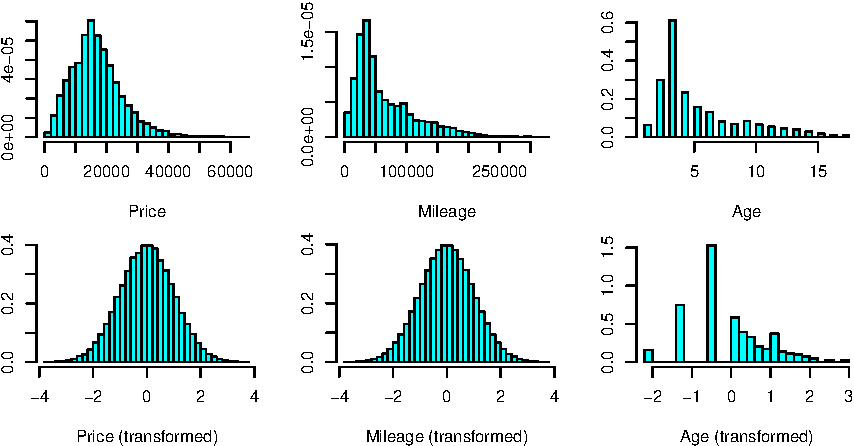
\includegraphics[width=4.2in,height=2.1in]{figs/hist_app-1} 

}

\caption[Distributions of car variables before and after normalization]{Distributions of car variables before and after normalization.}(\#fig:hist_app)
\end{figure}
\end{Schunk}

Next, we will fit a linear model on the transformed values of each
variable for our TBS regression. The reverse-transformation functions
will allow us to visualize how these variables affect model predictions
in terms of their original units.

\begin{Schunk}
\begin{Sinput}
p.t <- priceBN$x.t; m.t <- mileageBN$x.t; yo.t <- yearsoldBN$x.t
fit <- lm(p.t ~ m.t + yo.t)
\end{Sinput}
\end{Schunk}

\begin{Schunk}
<table class="table" style="width: auto !important; margin-left: auto; margin-right: auto;">
<caption>(\#tab:unnamed-chunk-11)TBS regression results for autotrader data.</caption>
 <thead>
  <tr>
   <th style="text-align:left;"> Variable </th>
   <th style="text-align:right;"> Estimate </th>
   <th style="text-align:right;"> Std. Error </th>
   <th style="text-align:right;"> t value </th>
   <th style="text-align:right;"> Pr(&gt;|t|) </th>
  </tr>
 </thead>
<tbody>
  <tr>
   <td style="text-align:left;"> Intercept </td>
   <td style="text-align:right;"> 0.005 </td>
   <td style="text-align:right;"> 0.010 </td>
   <td style="text-align:right;"> 0.553 </td>
   <td style="text-align:right;"> 0.58 </td>
  </tr>
  <tr>
   <td style="text-align:left;"> g(Mileage) </td>
   <td style="text-align:right;"> -0.234 </td>
   <td style="text-align:right;"> 0.016 </td>
   <td style="text-align:right;"> -14.966 </td>
   <td style="text-align:right;"> &lt; 0.001 </td>
  </tr>
  <tr>
   <td style="text-align:left;"> g(Age) </td>
   <td style="text-align:right;"> -0.441 </td>
   <td style="text-align:right;"> 0.016 </td>
   <td style="text-align:right;"> -27.134 </td>
   <td style="text-align:right;"> &lt; 0.001 </td>
  </tr>
</tbody>
</table>

\end{Schunk}

Unsurprisingly, we find that there are very significant relationships
between transformed car price, mileage, and age. However, to interpret
these values, we must resort to visualizations since there is no
inherent meaning of a ``one-unit increase'' in the ORQ normalized
measurements. We utilize the \CRANpkg{visreg} package \citep{visreg} to
perform our visualizations, using \code{predict.bestNormalize} in
conjunction with \pkg{visreg}'s \code{trans} and \code{xtrans} options
to view the relationship in terms of the original unit for the response
and covariate respectively (formatting
omitted).\footnote{Alternatively, one can use \CRANpkg{scales} \citep{scales} and \CRANpkg{ggplot2} \citep{ggplot2} to visualize any transformation fit using \pkg{bestNormalize}; instructions are included in the package vignette.}
For the sake of illustration, we have also plotted the estimated effect
of a generalized additive (spline) model fit with \CRANpkg{mgcv}
\citep{mgcv}.

\begin{Schunk}
\begin{Sinput}
visreg(fit, "m.t")
visreg(fit, "m.t", 
       partial = TRUE,
       trans = function(price.t) 
         predict(priceBN, newdata = price.t, inverse = TRUE)/1000, 
       xtrans = function(mileage.t) 
         predict(mileageBN, newdata = mileage.t, inverse = TRUE)
       )
\end{Sinput}
\end{Schunk}

\begin{Schunk}
\begin{figure}

{\centering 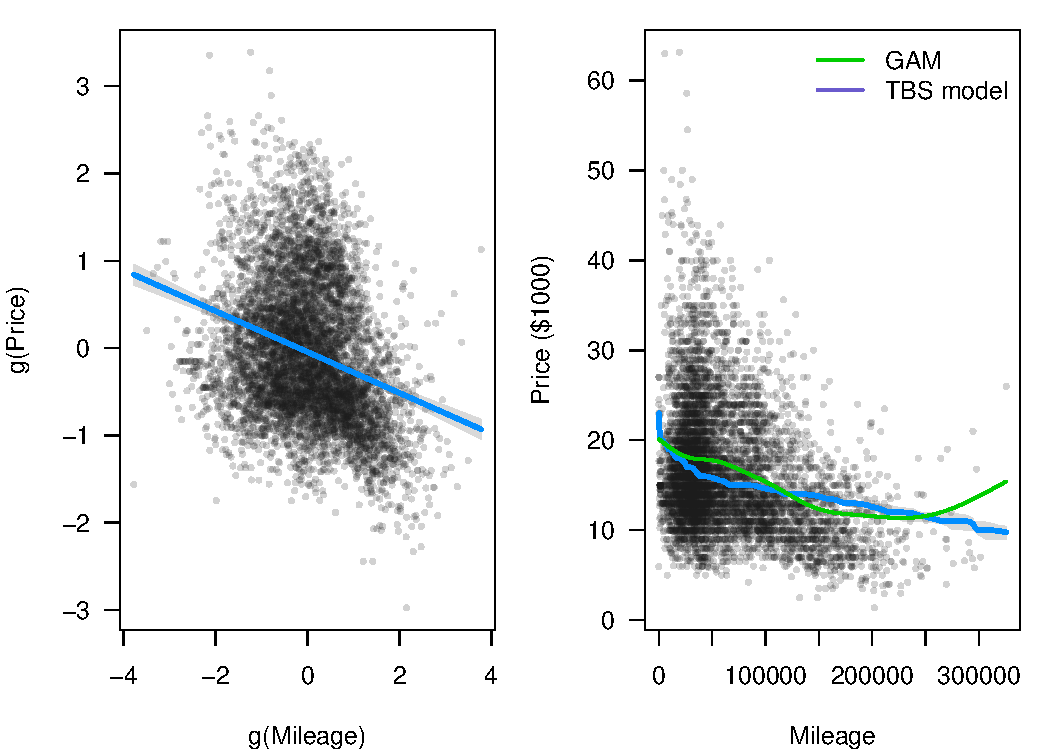
\includegraphics[width=0.8\linewidth]{figs/linear_visreg-1} 

}

\caption[TBS regression visualized on transformed units (left) and original units (right)]{TBS regression visualized on transformed units (left) and original units (right).}(\#fig:linear_visreg)
\end{figure}
\end{Schunk}

Below, we visualize the age effect, demonstrating how one might
visualize the effect outside of \pkg{visreg} (plot formatting is
omitted).

\begin{Schunk}
\begin{Sinput}
# Set up data for plotting line
new_yo <- seq(min(autotrader$yearsold), max(autotrader$yearsold), len = 100)
newX <- data.frame(yearsold = new_yo, mileage = median(autotrader$mileage))
newXt <- data.frame(yo.t = predict(yearsoldBN, newX$yearsold), 
                    m.t = predict(mileageBN, newX$mileage))

line_vals_t <- predict(fit, newdata = newXt) # Calculate line (transformed)
line_vals <- predict(priceBN, newdata = line_vals_t, inverse = TRUE)
plot(autotrader$yearsold, autotrader$price)
lines(new_yo, line_vals)
\end{Sinput}
\end{Schunk}

\begin{Schunk}
\begin{figure}

{\centering 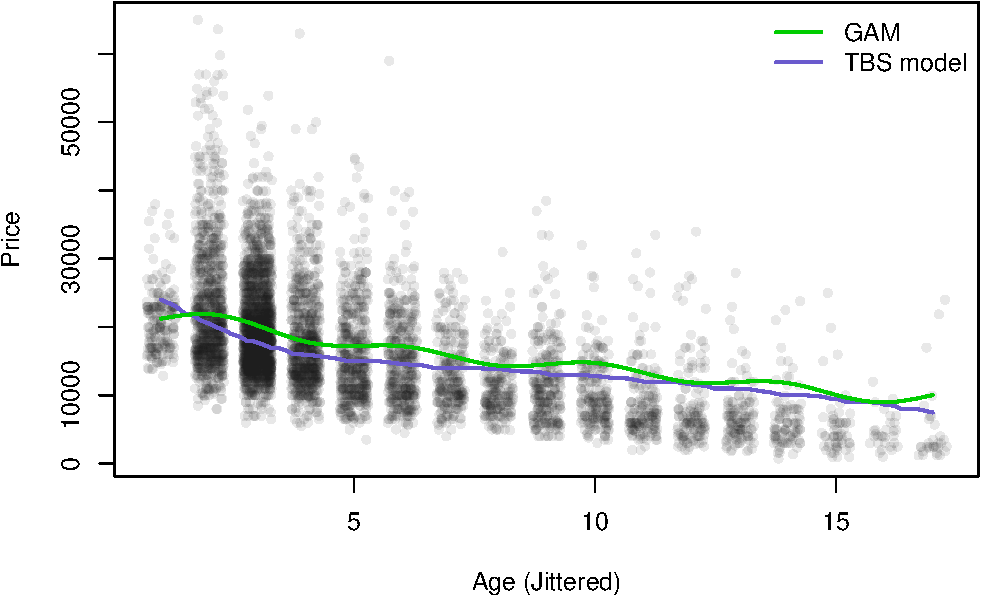
\includegraphics[width=0.8\linewidth]{figs/gam_tbs_model-1} 

}

\caption[Age effect on car price (re-transformed to original unit)]{Age effect on car price (re-transformed to original unit).}(\#fig:gam_tbs_model)
\end{figure}
\end{Schunk}

\hypertarget{implementation-with-recipes}{%
\subsection{Implementation with
recipes}\label{implementation-with-recipes}}

To build a predictive model for the price variable that uses each
vehicle's model and make in addition to its mileage and age, we can
utilize the \pkg{caret} and \pkg{recipes} functionality to do so. This
section outlines how to use \pkg{bestNormalize} in conjunction with
these other popular ML packages. Price is logged instead of ORQ
transformed in order to facilitate the interpretation of measures for
prediction accuracy.

\begin{Schunk}
\begin{Sinput}
library(tidymodels)
library(caret)
library(recipes)

set.seed(321)
df_split <- initial_split(autotrader, prop = .9)
df_train <- training(df_split)
df_test <- testing(df_split)

rec <- recipe(price ~ Make + model +  mileage + status + Year, df_train) %>% 
  step_mutate(years_old = 2017 - Year) %>% 
  step_rm(Year) %>% 
  step_log(price) %>% 
  step_best_normalize(all_predictors(), -all_nominal()) %>% 
  step_other(all_nominal(), threshold = 10) %>% 
  step_dummy(all_nominal()) %>% 
  prep()

fit1 <- train(price ~ ., bake(rec, NULL), method = 'glmnet')
fit2 <- train(price ~ ., bake(rec, NULL), method = 'earth')
fit3 <- train(price ~ ., bake(rec, NULL), method = 'rf')

r <- resamples(fits <- list(glmnet = fit1, earth = fit2, rf = fit3))
summary(r) # Extra-sample CV results
\end{Sinput}
\end{Schunk}

\begin{Schunk}
<table class="table" style="width: auto !important; margin-left: auto; margin-right: auto;">
<caption>(\#tab:unnamed-chunk-14)CV prediction accuracy of various ML methods.</caption>
 <thead>
  <tr>
   <th style="text-align:left;">   </th>
   <th style="text-align:right;"> Min. </th>
   <th style="text-align:right;"> 1st Qu. </th>
   <th style="text-align:right;"> Median </th>
   <th style="text-align:right;"> Mean </th>
   <th style="text-align:right;"> 3rd Qu. </th>
   <th style="text-align:right;"> Max. </th>
   <th style="text-align:right;"> NA's </th>
  </tr>
 </thead>
<tbody>
  <tr grouplength="3"><td colspan="8" style="border-bottom: 1px solid;"><strong>MAE</strong></td></tr>
<tr>
   <td style="text-align:left;padding-left: 2em;" indentlevel="1"> glmnet </td>
   <td style="text-align:right;"> 0.181 </td>
   <td style="text-align:right;"> 0.184 </td>
   <td style="text-align:right;"> 0.186 </td>
   <td style="text-align:right;"> 0.189 </td>
   <td style="text-align:right;"> 0.194 </td>
   <td style="text-align:right;"> 0.198 </td>
   <td style="text-align:right;"> 0 </td>
  </tr>
  <tr>
   <td style="text-align:left;padding-left: 2em;" indentlevel="1"> earth </td>
   <td style="text-align:right;"> 0.147 </td>
   <td style="text-align:right;"> 0.151 </td>
   <td style="text-align:right;"> 0.154 </td>
   <td style="text-align:right;"> 0.155 </td>
   <td style="text-align:right;"> 0.158 </td>
   <td style="text-align:right;"> 0.163 </td>
   <td style="text-align:right;"> 0 </td>
  </tr>
  <tr>
   <td style="text-align:left;padding-left: 2em;" indentlevel="1"> rf </td>
   <td style="text-align:right;"> 0.136 </td>
   <td style="text-align:right;"> 0.141 </td>
   <td style="text-align:right;"> 0.143 </td>
   <td style="text-align:right;"> 0.144 </td>
   <td style="text-align:right;"> 0.147 </td>
   <td style="text-align:right;"> 0.157 </td>
   <td style="text-align:right;"> 0 </td>
  </tr>
  <tr grouplength="3"><td colspan="8" style="border-bottom: 1px solid;"><strong>RMSE</strong></td></tr>
<tr>
   <td style="text-align:left;padding-left: 2em;" indentlevel="1"> glmnet </td>
   <td style="text-align:right;"> 0.242 </td>
   <td style="text-align:right;"> 0.247 </td>
   <td style="text-align:right;"> 0.252 </td>
   <td style="text-align:right;"> 0.256 </td>
   <td style="text-align:right;"> 0.264 </td>
   <td style="text-align:right;"> 0.276 </td>
   <td style="text-align:right;"> 0 </td>
  </tr>
  <tr>
   <td style="text-align:left;padding-left: 2em;" indentlevel="1"> earth </td>
   <td style="text-align:right;"> 0.203 </td>
   <td style="text-align:right;"> 0.209 </td>
   <td style="text-align:right;"> 0.214 </td>
   <td style="text-align:right;"> 0.217 </td>
   <td style="text-align:right;"> 0.226 </td>
   <td style="text-align:right;"> 0.235 </td>
   <td style="text-align:right;"> 0 </td>
  </tr>
  <tr>
   <td style="text-align:left;padding-left: 2em;" indentlevel="1"> rf </td>
   <td style="text-align:right;"> 0.193 </td>
   <td style="text-align:right;"> 0.208 </td>
   <td style="text-align:right;"> 0.213 </td>
   <td style="text-align:right;"> 0.210 </td>
   <td style="text-align:right;"> 0.215 </td>
   <td style="text-align:right;"> 0.217 </td>
   <td style="text-align:right;"> 0 </td>
  </tr>
  <tr grouplength="3"><td colspan="8" style="border-bottom: 1px solid;"><strong>RSQ</strong></td></tr>
<tr>
   <td style="text-align:left;padding-left: 2em;" indentlevel="1"> glmnet </td>
   <td style="text-align:right;"> 0.767 </td>
   <td style="text-align:right;"> 0.772 </td>
   <td style="text-align:right;"> 0.785 </td>
   <td style="text-align:right;"> 0.782 </td>
   <td style="text-align:right;"> 0.789 </td>
   <td style="text-align:right;"> 0.801 </td>
   <td style="text-align:right;"> 0 </td>
  </tr>
  <tr>
   <td style="text-align:left;padding-left: 2em;" indentlevel="1"> earth </td>
   <td style="text-align:right;"> 0.807 </td>
   <td style="text-align:right;"> 0.833 </td>
   <td style="text-align:right;"> 0.845 </td>
   <td style="text-align:right;"> 0.842 </td>
   <td style="text-align:right;"> 0.855 </td>
   <td style="text-align:right;"> 0.864 </td>
   <td style="text-align:right;"> 0 </td>
  </tr>
  <tr>
   <td style="text-align:left;padding-left: 2em;" indentlevel="1"> rf </td>
   <td style="text-align:right;"> 0.835 </td>
   <td style="text-align:right;"> 0.845 </td>
   <td style="text-align:right;"> 0.855 </td>
   <td style="text-align:right;"> 0.854 </td>
   <td style="text-align:right;"> 0.860 </td>
   <td style="text-align:right;"> 0.873 </td>
   <td style="text-align:right;"> 0 </td>
  </tr>
</tbody>
</table>

\end{Schunk}

Evidently, the random forest generally performed better in
cross-validated prediction metrics, achieving a higher R-squared (RSQ),
lower root-mean-squared error (RMSE), and lower mean absolute error
(MAE). Since price was logged, RMSE and MAE are on the log scale. For
the test set, we calculate these quantities in price's original unit
(2017 US dollars) using the \CRANpkg{yardstick} package
\citep{yardstick}.

\begin{Schunk}
\begin{Sinput}
# Out of sample prediction accuracy
results <- lapply(fits, function(x) {
  p <- c(predict(x, newdata = bake(rec, df_test)))
  yardstick::metrics(data.frame(est = exp(p), truth = df_test$price), 
                     truth = truth, estimate = est)
})
results
\end{Sinput}
\end{Schunk}

\begin{Schunk}
<table class="table" style="width: auto !important; margin-left: auto; margin-right: auto;">
<caption>(\#tab:unnamed-chunk-16)Test data prediction accuracy of various ML methods. RMSE and MAE can be interpreted in terms of 2017 US dollars.</caption>
 <thead>
  <tr>
   <th style="text-align:left;"> Method </th>
   <th style="text-align:right;"> RMSE </th>
   <th style="text-align:right;"> RSQ </th>
   <th style="text-align:right;"> MAE </th>
  </tr>
 </thead>
<tbody>
  <tr>
   <td style="text-align:left;"> glmnet </td>
   <td style="text-align:right;"> 4076 </td>
   <td style="text-align:right;"> 0.772 </td>
   <td style="text-align:right;"> 2847 </td>
  </tr>
  <tr>
   <td style="text-align:left;"> earth </td>
   <td style="text-align:right;"> 3619 </td>
   <td style="text-align:right;"> 0.814 </td>
   <td style="text-align:right;"> 2500 </td>
  </tr>
  <tr>
   <td style="text-align:left;"> rf </td>
   <td style="text-align:right;"> 3257 </td>
   <td style="text-align:right;"> 0.853 </td>
   <td style="text-align:right;"> 2294 </td>
  </tr>
</tbody>
</table>

\end{Schunk}

After normalization of mileage and age, a random forest had the optimal
predictive performance on car price given a car's make, model, age, and
mileage compared to other ML models, achieving out-of-sample R-squared
0.853 on a left-out test data set. We conjecture that the random forest
performs best because it can better capture differential depreciation by
make and model than the other methods.

\hypertarget{discussion}{%
\section{Discussion}\label{discussion}}

We have shown how the \pkg{bestNormalize} package can effectively and
efficiently find the best normalizing transformation for a vector or set
of vectors. However, normalization is by no means something that should
be applied universally and without motivation. In situations where units
have meaning, normalizing prior to analysis can contaminate the
relationships suspected in the data and/or reduce predictive accuracy.
Further, depending on the type of transformations used, interpreting
regression coefficients post-transformation can be difficult or
impossible without using a figure since the transformation function
itself will look completely different for different distributions. So,
while normalization transformations may well be able to increase the
robustness of results and mitigate violations to the classical linear
regression assumption of Gaussian residuals, it is by no means a
universal solution.

On the other hand, when hypotheses are exploratory or when data is of
poor quality with high amounts of skew/outliers, normalization can be an
effective means of mitigating downstream issues this can cause in the
analyses. For example, in machine learning contexts, some predictor
manipulations rely on second-order statistics (e.g., principal
components analysis or partial least squares), for which the variance
calculation can be sensitive to skew and outliers. Normalizing
transformations can improve the quality and stability of these
calculations. Similarly, predictor normalization reduces the tendency
for high-leverage points to have their leverage propagated into
engineered features such as interactions or polynomials. Ultimately,
these benefits can often produce predictive models that are more robust
and stable.

We focused on making this package useful in a variety of machine
learning workflows. We are enthusiastic in our support of
\pkg{bestNormalize}, and will continue to maintain the package while it
is found to be useful by R users. We hope to continue to build up the
repertoire of candidate transformations using the same infrastructure so
that additional ones can be considered by default in the future.

\hypertarget{references}{%
\section{References}\label{references}}

\begin{verbatim}
\end{verbatim}

\bibliography{RJournal-final-submission.bib}

\address{%
Ryan A. Peterson\\
Department of Biostatistics and Informatics\\%
University of Colorado Anschutz Medical Campus 13001 East 17th Place
Aurora, Colorado 80045 ORCID: 0000-0002-4650-5798\\
%
\url{https://petersonr.github.io/}\\%
%
\email{ryan.a.peterson@cuanschutz.edu}%
}
